\section{Confidenzialità e integrità delle query}
Garantire la privacy dei dati pubblicati protegge la confidenzialità dei dati (confidenzialità del contenuto) come anche l'accesso agli stessi:
\begin{itemize}
    \item \textbf{confidenzialità di accesso}: riservatezza del fatto che un accesso mira a un dato specifico
    \item \textbf{confidenzialità di pattern}: riservatezza del fatto che due accessi mirano agli stessi dati
\end{itemize}
Esistono diversi approcci per proteggere l'accesso ai dati e nelle prossime sezioni andremo ad approfondirne alcuni.
\subsection{Path ORAM}
L'idea che sta alla base è quella di eseguire query senza dire al server cosa sto cercando. \\
Lato \textbf{server}: i dati sono organizzati in un albero binario, dove ciascun nodo è un blocco dove metto dentro più cose (dati reali e spazio, dummy blocks) e dove c’è un unico cammino che va dalla foglia alla radice.\\
Lato \textbf{client}: si tiene un po' di memoria localmente (stash), si tiene una mappa delle chiavi (in che posizione è mappata la chiave). Se il blocco esiste, sta da qualche parte nel cammino dalla radice alla posizione della chiave. La mappa di posizionamento cambia ogni volta che si accede o si rimappa un blocco.\\
In ogni momento ogni blocco è mappato uniformemente e in maniera randomica in un bucket delle foglie e blocchi unstashed sono posizionati sempre in qualche bucket lungo il percorso che va alla foglia mappata.\\
Le operazioni che possiamo fare sono:
\begin{enumerate}
    \item rimappare i blocchi: sia x la vecchia posizione di a. Si rimappa randomicamente la posizione di a in una nuova posizione (un nuovo nodo foglia)
    \item leggere il percorso: legge i nodi che in P(x) contengono a. Se l'accesso è una scrittura si aggiorna il dato salvato nel blocco a.
    \item scrivere il percorso: scrive i nodi in P(x) includendo qualche blocco aggiuntivo dallo stash se possono essere inclusi nel percorso (deve essere verificata l'invariante principale)
\end{enumerate}
Vediamo un esempio:
\begin{center}
    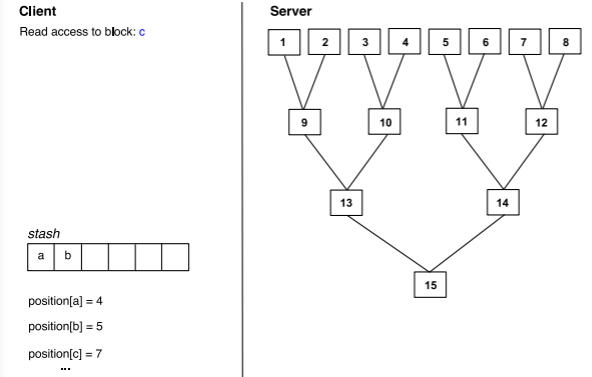
\includegraphics[scale=0.8]{img/poram.png}
\end{center}
La posizione di a è 4: significa che a si trova da qualche parte lungo il cammino dalla radice al bucket 4. Il client si tiene il dizionario per tutte le chiavi. Lo stash è come se fosse una cache locale. Ogni volta che qualcuno legge una cosa, cambi il posto. Così se un altro utente andrà a leggere la stessa cosa, avrà un percorso diverso. Come funziona l’accesso?\\
L'utente vuole leggere il valore di una certa chiave
\begin{center}
    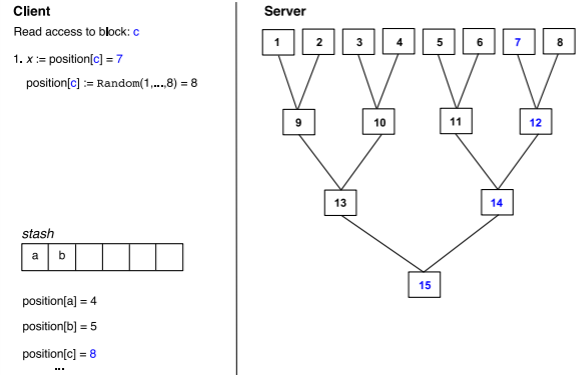
\includegraphics[scale=0.8]{img/poram1.png}
\end{center}
Leggo il cammino a cui trovo c
\begin{center}
    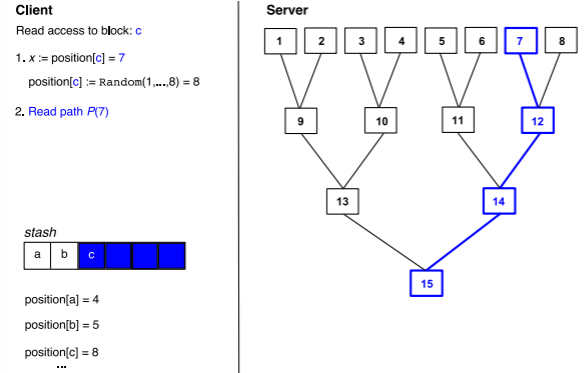
\includegraphics[scale=0.8]{img/poram2.png}
\end{center}
Leggendo scarico il più possibile la mia stash (elenco di cose che ho letto ma che devo ancora riscrivere). Cioè già che faccio quel percorso, mappo nel percorso le lettere che sono ancora nella stash.
\begin{center}
    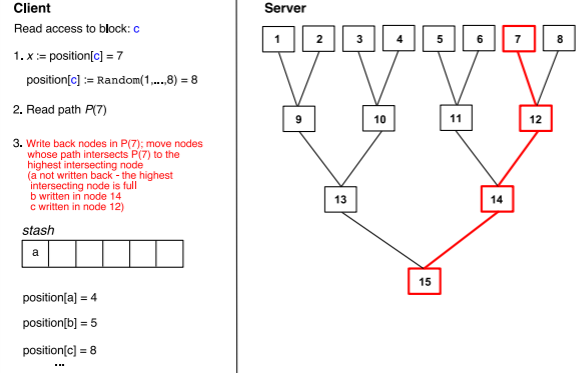
\includegraphics[scale=0.8]{img/poram3.png}
\end{center}
\textbf{Problema di Path ORAM}: ogni lettura, che solitamente non è concorrente, diventa anche scrittura, che invece è concorrente. Quindi diventa pesante, soprattutto se ci sono tanti accessi multipli.
\subsection{Ring ORAM}
Variazione di Path ORAM che riduce l'accesso alla banda online a O(1). All'interno dei nodi ho: dei blocchi addizionali, una piccola mappa degli offsets dei blocchi, un contatore degli accessi.\\
La lettura è a livello dei singoli blocchetti, quindi vengono letti anche i blocchetti vuoti. Il contatore serve per fare in modo che la lettura di questi blocchetti vuoti non venga scoperta.
Non scrive tutte le volte che va a leggere ma solo quando i contatori dicono che le letture potrebbero diventare osservabili. 

\subsection{Shuffle Index}
La questione di base è sempre quella: se voglio proteggere la privacy devo rompere il legame tra il dato e la posizione del dato.\\
Lato \textbf{client}: organizzo le chiavi come un albero di ricerca, non un albero binario ma un albero paginato (B+). Però in questo caso le foglie non sono collegate (chained) ma sono scollegate (unchained) perché così le posso mischiare (shuffle). Anche perché il puntatore delle foglie può fare leakage del fatto che una foglia viene prima di un’altra.\\
I nodi hanno la seguente struttura:
\begin{itemize}
    \item ciascun nodo deve essere riempito almeno della metà della sua capienza, così da riempire bene l’albero
    \item l’i-esimo figlio è la radice del sottoalbero che contiene i nodi v tali per cui i figli stanno tra le due chiavi (\(\geq\))
\end{itemize}
\begin{center}
    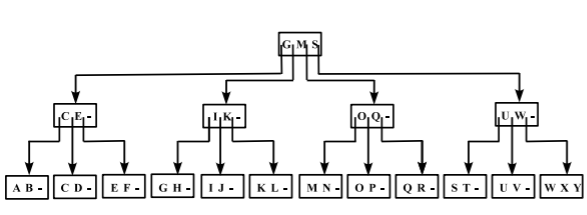
\includegraphics[scale=0.8]{img/shuffle.png}
\end{center}
\subsubsection{Rappresentazione a livello logico}
I puntatori tra i nodi della struttura astratta corrispondono (a livello logico) agli identificatori dei nodi.\\
Sono rappresentati da un insieme di coppie \(\langle id, n \rangle\) con id che è l'identificatore e n il contenuto del nodo: l'ordine tra gli identificatori non corrisponde necessariamente all'ordine in cui i nodi appaiono nella rappresentazione astratta
\begin{center}
    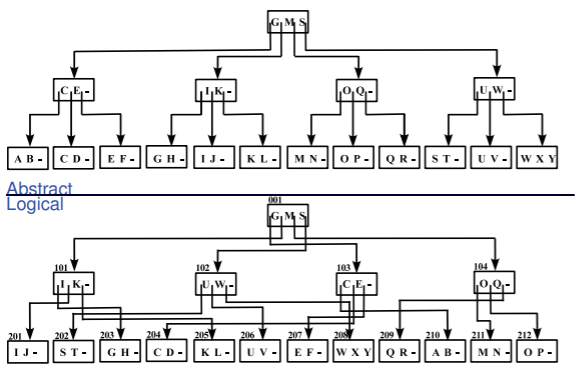
\includegraphics[scale=0.8]{img/abslog.png}
\end{center}
\subsubsection{Rappresentazione a livello fisico}
Ogni nodo \(\langle id, n \rangle\) nello shuffle index a livello logico è salvato sul server in maniera criptata.\\
Ogni nodo \(\langle id, n \rangle\) corrisponde a un blocco \(\langle id, b \rangle\) dove b è un blob che contiene il contenuto criptato con la sua firma e un sale random così che ogni criptazione sia diversa. Alla fine un MAC con chiave cripta il contenuto con l’identificatore, perché non posso spostare a caso il contenuto dei nodi.\\
Quindi: cripto il contenuto delle foglie, lo concateno con il suo id e faccio un hash con chiave per firmare (id, b).
\begin{center}
    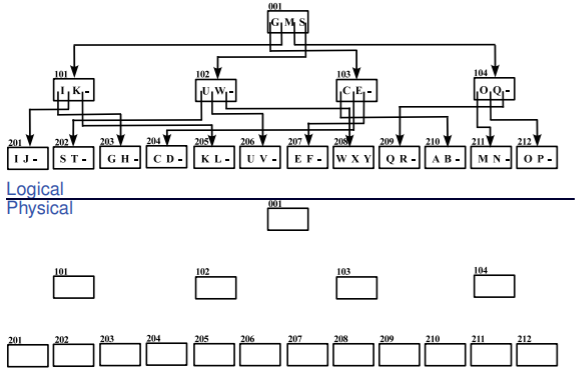
\includegraphics[scale=0.8]{img/logfis.png}
\end{center}
Avendo tutto criptato, non è il server che mi dice quale puntatore seguire. Dovrà farlo il client decriptato il nodo.
\subsubsection{Accesso ai dati}
Accedere ai dati richiede un processo iterativo tra client e server. Il client esegue un'iterazione per ogni livello di shuffle index partendo dalla radice. Ad ogni iterazione il client:
\begin{itemize}
    \item decripta il blocco ricevuto
    \item determina il blocco che deve essere recuperato dal server al prossimo livello
\end{itemize}
Il processo termina quando viene recuperato un blocco foglia.
\begin{center}
    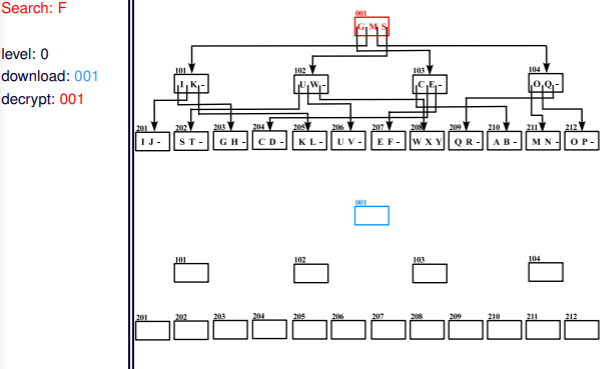
\includegraphics[scale=0.8]{img/shuffleaccess.png}
\end{center}
\begin{center}
    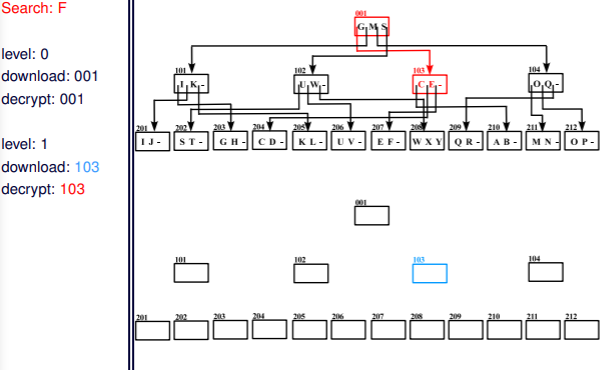
\includegraphics[scale=0.8]{img/shuffleaccess1.png}
\end{center}
\begin{center}
    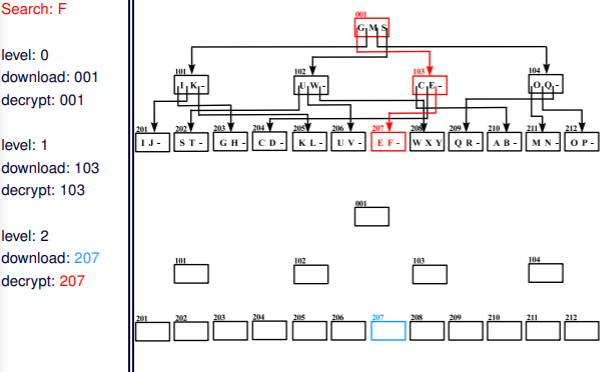
\includegraphics[scale=0.8]{img/shuffleaccess2.png}
\end{center}
Il server riceve un insieme di blocchi da salvare e le richieste di accedere ai blocchi che vengono tradotte in osservazioni: un'osservazione \(o_i\) corrisponde a una sequenza di blocchi.\\
Il server può quindi fare molto facilmente inferenze su:
\begin{itemize}
    \item il numero m di blocchi e i loro identificatori
    \item l'altezza h del shuffle index
    \item il livello associato ad ogni blocco
\end{itemize}
Data una sequenza di osservazioni il server non dovrebbe essere capace di effettuare inferenze su:
\begin{itemize}
    \item dati salvati nel shuffle index (confidenzialità del contenuto)
    \item l'accesso ai dati si riferisce ad un nodo specifico (confidenzialità di accesso)
    \item \(o_i\) ha lo scopo di accedere allo stesso nodo di \(o_j\) (confidenzialità di pattern)
\end{itemize}
La criptazione lato server protegge la confidenzialità del contenuto e la confidenzialità dell'accesso per ogni richiesta individuale. \\
Tuttavia non vengono protetti confidenzialità di accesso e pattern dato che accedere agli stessi blocchi implica accedere agli stessi dati. Si possono eseguire attacchi di frequenza che permettono di ricostruire la corrispondenza tra il valore degli attributi in chiaro e i blocchi.\\
Per distruggere questa corrispondenza si combinano tre strategie:
\begin{enumerate}
    \item \textbf{cover searches}: aggiungo rumore (mi interessa una chiave ma ne aggiungo altre alla ricerca)
    \item \textbf{cached searches}: tengo qualche informazione lato client
    \item \textbf{shuffling}: cambia dinamicamente l'allocazione dei blocchi ad ogni accesso
\end{enumerate}
\subsubsection{Cover searches}
Introduco confusione aggiungendo richieste di cui in realtà non mi importa.\\
Il numero di coperture (num\_cover) è un parametro di protezione.\\
Questa strategia deve:
\begin{itemize}
    \item fornire una diversità tra i blocchi (differenza tra i percorsi dei blocchi che mi interessano e i blocchi che introducono rumore)
    \item essere indistinguibile dalla ricerca effettiva
\end{itemize}
\begin{center}
    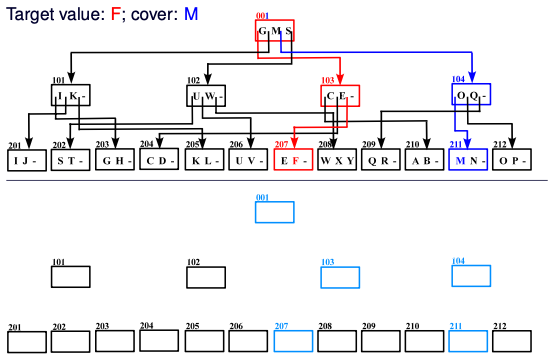
\includegraphics[scale=0.5]{img/coversearch.png}
\end{center}
Potremmo subire attacchi di inserzione: la query vera rimane sempre uguale mentre quella di copertura cambia ogni volta.

\subsubsection{Cached searches}
Il client mantiene una cache locale con gli ultimi accessi effettuati.\\
Se c’è un nodo in cache allora anche suo padre deve stare in cache (path continuity).\\
La cache cambia ad ogni accesso.\\
Se un nodo è nella cache posso o non fare nulla o fare ricerca cover.\\
Questo metodo protegge dagli attacchi di inserzione a breve termine, mentre può essere soggetto ad attachi di inserzione che vanno oltre la dimensione della cache.

\subsubsection{Shuffling}
Questa tecnica va a rompere la corrispondenza uno a uno tra blocchi e nodi, cambiando il contenuto tra i nodi. \\Il shuffling richiede decryption e re-encryption: ad ogni spostamento il nodo va recriptato con un sale diverso. Se cambio i nodi devo anche cambiare il puntatore verso i genitori.\\\\

Prendendo in considerazione tutte e tre le tecniche abbiamo:
\begin{itemize}
    \item degradazione dovuta allo shuffling
    \item confidenzialità di accesso: ogni volta che viene fatto l'accesso a un'informazione viene aggiunto un rumore che distrugge la corrispondenza nodo-blocco
    \item confidenzialità di pattern: a breve termine con cover e cache, a lungo termine con cover e shuffling
\end{itemize}
È sicuramente un metodo molto costoso: num\_cover + num\_cache + una scrittura sul server. Ha prestazioni migliori di Path ORAM